\documentclass[10pt]{beamer}
\usepackage{pgfpages}
\hypersetup{pdfpagemode=FullScreen}
% \setbeameroption{show notes on second screen}

% \documentclass[notes=only]{beamer}   % only notes
% \documentclass[notes]{beamer}       % print frame + notes
%\documentclass{beamer}              % only frames

\usetheme[progressbar=frametitle]{metropolis}

\usepackage{booktabs}
\usepackage[scale=2]{ccicons}

\usepackage{pgfplots}
\usepgfplotslibrary{dateplot}

\usepackage{xspace}
\newcommand{\themename}{\textbf{\textsc{metropolis}}\xspace}

\title{Dynamic Scalable State Machine Replication}
%\subtitle{A modern beamer theme}
\date{\today}
\author{
  Long Hoang Le\\
  \texttt{}\\
  \and
  Eduardo Bezerra\\
  \texttt{}\\
  \and
  Fernando Pedone\\
  \texttt{}}
  
\institute{Università della Svizzera italiana}
% \titlegraphic{
\includegraphics[height=1.5cm]{figures/logo}}

\begin{document}

\maketitle

\note[itemize]{
\item Good morning everyone, my name is Long, I'm a PhD student from university of Lugano, Switzerland., and it's such an honor for me to be here today to present about our work, which is called Dynamic Scalable State Machine Replication.
\item This is a joint work between me, Eduardo Bezerra and prof. Fernando Pedone, both also come from university of lugano.
}

\begin{frame}{Outlines}
  \setbeamertemplate{section in toc}[sections numbered]
  \tableofcontents[hideallsubsections]
\end{frame}

\note[itemize]{
\item So this is the outline of my presentation today. I'll talk a little bit about our motivation, as well as giving you some background information of the state of the art, 
\item Then I'll talk about the idea of dynamic scalable state machine replication which is our work, how we implemented that idea, and how we evaluated it, in terms of perfomance, 
and few words of conclusion.
}

\section{Motivation}

\note[itemize]{
\item OK, let's start with the motivation.
}

\begin{frame}[fragile]{The need of availability}

  \begin{figure}
    % \includegraphics<1>[width=.8\textwidth]{figures/smr-1}
    % \includegraphics<2>[width=.8\textwidth]{figures/smr-2}
    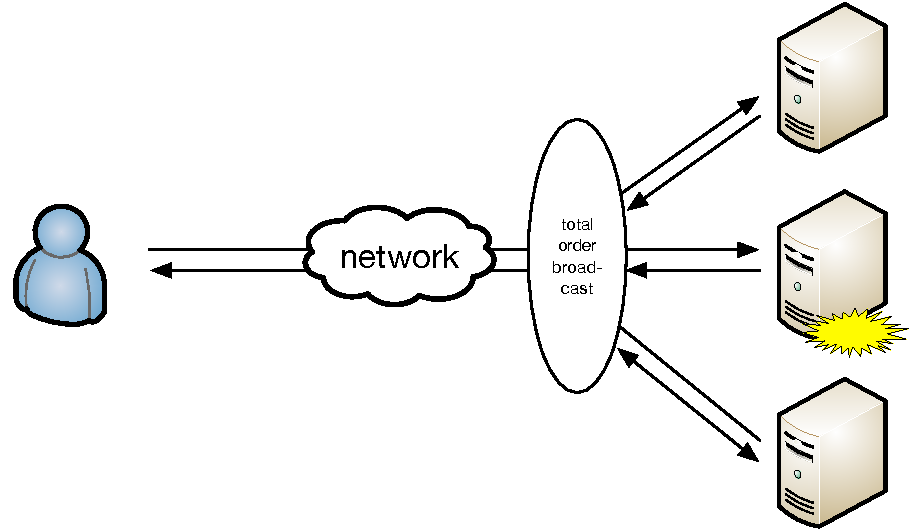
\includegraphics[width=.8\textwidth]{figures/smr-3}
  \end{figure}
\end{frame}

\note[itemize]{
\item  Nowadays, people incorporate many online services into their life and heavily depend on those services, so people want them to be available all the time. Suppose you are a service provider, and you have an online application or service that you want to make reliable, fault tolerance. One way to do that is executing that application on a collection of machine and ensure that they all execute commands in the same way, to reach the same result. So if one or even more machine is down, the system still works properly, as long as the majority of the machine is fine. So that's the main idea of state machine replication
}

\begin{frame}[fragile]{State Machine Replication (SMR)}

  Providing fault-tolerance, strong consistency
  \begin{itemize}
    \item All replicas start in the same initial state
    \item Apply same set of commands in the same order 
    \item The executions of commands are deterministic
    \item Proceed through the same set of states
  \end{itemize}
\end{frame}

\note[itemize]{
\item So, State Machine Replication SMR provides fault-tolerance, strong consistency by ensuring following criteria:
  \begin{itemize}
    \item All replicas of the service/application start in the same initial state
    \item and all replica apply same set of commands in the same order. To ensure this, SMR relies on a total order broadcast primitive
    \item The executions of commands must be deterministic, which means that with the same input, all the replica have to produce the same output. None of them can give any arbitrary output
    \item so by doing that all replicas will go through the same set of states
  \end{itemize}
}

\begin{frame}[fragile]{State Machine Replication}
  Production systems
  % Many production systems use this approach to tolerate crash faults:
  \begin{itemize}
    \item Keep critical managements service online
    \begin{itemize}
      \item Google's Chubby, Apache Zookeeper
    \end{itemize}
    \item Persistent storage in distributed databases
    \begin{itemize}
      \item Google Spanner, Windows azure storage, CockroachDB, Apache H-Store
    \end{itemize}
  \end{itemize}
\end{frame}

\note[itemize]{
\item So far, more and more production systems use state machine replication as a solution for increasing availability. For example, Google's Chubby and Apache Zookeeper are used as distributed lock manager for keeping critical managements service online. Or we can name many distributed storage and databases, such as google spanner, azure storage, apache h-store and so on
} 

\begin{frame}[fragile]{Scaling State Machine Replication}

  SMR lacks of scalability:
  \begin{itemize}
    \item Every replica executes all commands.
    \item Adding servers does not increase the maximum throughput
  \end{itemize}
  
  Different techniques have been developed to deal with these limitations
  \begin{itemize}
    \item Scaling up
    \item Scaling out
  \end{itemize}

\end{frame}

\note[itemize]{
\item In today’s world where large-scale applications are commonplace, scalability is the key. The system must be able to handle massive throughput. However in terms of throughput, SMR doesn't scale, because:
  \begin{itemize}
    \item Every replica has to execute all commands, in order to reach to same state
    \item So, adding more servers does not increase the maximum throughput
  \end{itemize}
\item So, different techniques have been proposed for scaling SMR
  \begin{itemize}
    \item Some works propose Scaling up technique that takes advantage of multiple cores to execute requests in parallel. Although effective, the improvements are limited by the number of cores available on servers. 
    \item And Scaling out is another technique the divides application's state in to smaller partitions, and have some mechanism to ensure consistency of the system.
  \end{itemize}
}

\begin{frame}[fragile]{Scalable State Machine Replication (SSMR)}
    \uncover<1-> {Partitions application's state and replicates each partition}

    \includegraphics<2>[width=1\textwidth]{figures/ssmr-local}
    \includegraphics<3->[width=1\textwidth]{figures/ssmr-global}

    \uncover<4-> {Guarantees strong consistency (i.e., linearizability)}

    \uncover<5-> {\alert {Expensive cost of multi-partition commands}}

    \uncover<6-> {\alert{Assumes a static workload partitioning}}

    \note<1>{
      In the scope of this work, we will mainly focus on the second direction, which is dividing application states into smaller part, and host them on multiple partition. Scalable state machine replication (SSMR) was proposed as an implementation in this direction
    }
    \note<2>{
      for example, if an application has 2 variables X and Y, we can put X on one partition, say PX, and Y on another one, say PY. So whenever there is a command accesses X, that command will only be sent to partition PX which is holding X. So PX will calculate and response to that command, while partition PY will still be free to serve other commands. Thus we can scale the system by adding more partition.
    }
    \note<3>{
      In the case of command that accesses both X and Y, PX and PY will have to communicate in the way that one must send the other the variable it's holding, and inform the other when it start the execution. 
    }
    \note<4>{
      By having partition exchanging signal, SSMR also guarantees strong consistency at linearizability level.
    }
    \note<5>{
      However SSMR still has some weaknesses, due to its implementation. Firstly, With globals commands, partitions have to exchange the data and signal, all partitions have to wait for the others. Then adding more partition doesn't really increase the throughput of the system, because it also increases the cost of global command, since partition have to wait for more exchanged data.
    }
    \note<6>{
      Secondly, because client has to be able to determine the target partition to send command to, the whole SSMR system has to rely on a static workload partitioning. any state reorganization requires system shutdown and manual modification.
    }

\end{frame}



\section{Dynamic Scalable State Machine Replication}

\note[itemize]{
\item By addressing those problems with current implementation of scalability of state machine replication, we came up with the idea of what is called dynamic scalable state machine replication 
}

\begin{frame}{System Model}
  Crash-stop failure model
  \begin{itemize}
    \item No Byzantine behavior
  \end{itemize}

  Communication by message passing
  \begin{itemize}
    \item One-to-one communication use reliable multicast
    \item One-to-many communication relies on atomic multicast
    \item Messages can be lost, reordered, but not corrupted
  \end{itemize}

  System is partially synchronous
  \begin{itemize}
    \item No delay bound
  \end{itemize}

  Consistency level: linearizability
\end{frame}

\note[itemize]{
\item First, let's go through the system model.
In our system, we consider set of client and server processes, process is either correct, if they never fail, othwerise, crashed. In either case, processes do not have abitary behavior.

Processes communicate by message passing. using either one to one (which is based on reliable multicast), or one to many communication (rely on atomic multicast). Messages can be lost, reordered, but not corrupted.

The system is asynchronous: there is no bound on message delay or on relative process speed

And our consistency creterion is linearizability, which is a strong consistency level, 
}


\begin{frame}{General idea}
  Dynamically changing the state partitioning by exploiting locality

  \begin{itemize}
    \item Involved variables are moved to a single partition
    \item Command is executed against this partition
    \item Supported commands: $consult, create, access, move, delete$
  \end{itemize}

  Variables that are usually accessed together are moved to the same partition

  Variable mapping managed by an Oracle partition and client cache

  DS-SMR falls back to S-SMR execution after few unsuccessful attempts.

\end{frame}

\note[itemize]{
\item So, the main idea of DSSMR is Dynamically reconfigure state partitioning on the fly, by exploiting workload locality. Our scheme benefits from simple case, like commands that repeatedly access same state variables, and more complex case, such as social network applications, where users with common interests have a higher probability of interaction.Focusing on locality allows us to have a simple but effective approach to state reconfiguration: whenever a command requires data from multiple partitions, the variables involved are moved to a single partition and the command is executed against this partition.

\item So variable will be moved among partitions, but eventually, variables that are often accessed together will converge on a same partition. Then the command that access those variable would become a single partition command.

\item To track object locations, we have a centralized oracle that contains accurate information about the location of state variables, and in addition, each client stores to local cache the previous consult to the Oracle. To ensure that commands always succeed, after attempting to execute a command a few times unsuccessfully, DS-SMR retries the command using S-SMR’s execution and involving all partitions

}

% \begin{frame}{General idea}
  
%   Clients query the oracle to know each variable's location

%   Clients moves variables if necessary, then execute command on that partition 

%   Clients $retry$ if variables change location

%   Clients fall back to S-SMR after a number of retries

% \end{frame}

% \note[itemize]{
% \item So, in order to execute a command, clients first query the oracle to know each the location of involve variable. Then it will try to move all variables to one partition, then execute the command on that partition. 

% if the variable changed location during the execution, the client will retry command.

% There could be a case that many clients try to move same variable to different partitions, so in order to guarantee the termination of the algorithm, client fall back to the original SSMR execution after a number of retries, which mean that client will send that command to all involved partition.
% }

\begin{frame}{General idea}
  \begin{figure}
    \includegraphics<1>[width=1\textwidth]{figures/dssmr-1-1}
    \includegraphics<2>[width=1\textwidth]{figures/dssmr-1-2}
    \includegraphics<3>[width=1\textwidth]{figures/dssmr-1-3}
    \includegraphics<4>[width=1\textwidth]{figures/dssmr-2-0}
    \includegraphics<5>[width=1\textwidth]{figures/dssmr-2-1}
    \includegraphics<6>[width=1\textwidth]{figures/dssmr-2-2}
    \includegraphics<7>[width=1\textwidth]{figures/dssmr-2-3}
    \includegraphics<8>[width=1\textwidth]{figures/dssmr-2-4}
    \includegraphics<9>[width=1\textwidth]{figures/dssmr-2-5}
  \end{figure}
  \note<1>{
    Let's consider an example execution of DSSMR. In this scenario, we have 2 clients a and b, and a variable: X is on partition P1. 
  }
  \note<2>{
    client a wants to read value of X, first it will consult the oracle for x's location. Oracle will return that x is on P1, so client a send the read command to P1.
  }
  \note<3>{
    client a wants to read value of X, first it will consult the oracle for x's location. Oracle will return that x is on P1, so client a send the read command to P1.
  }
  \note<4>{
    then after a while, a wants to read x again, it does the similar step: query oracle for x's location, oracle tell x is on p1. 
  }
  \note<5>{
    then after a while, a wants to read x again, it does the similar step: query oracle for x's location, oracle tell x is on p1. 
    
  }
  \note<6>{
   But right before c1 send read command to P1, another client B does the move X to p2.
    
  }
  \note<7>{
  so when C1 send read to P1, the partition will tell the client to retry. 
    
  }
  \note<8>{
  Then client a have to do the process again: consulting the oracle to get x's location which is p2 now, then send read command to p2.
  }
  \note<9>{
  
  }
\end{frame}

\note[itemize]{
\item Let's consider an example execution of DSSMR. In this scenario, we have 2 clients a and b, and a variable: X is on partition P1. 
  
  client a wants to read value of X, first it will consult the oracle for x's location. Oracle will return that x is on P1, so client a send the read command to P1.

  then after a while, a wants to read x again, it does the similar step: query oracle for x's location, oracle tell x is on p1. But right before c1 send read command to P1, another client B does the move X to p2. so when C1 send read to P1, the partition will tell the client to retry. Then client a have to do the process again: consulting the oracle to get x's location which is p2 now, then send read command to p2.
}

\begin{frame}{Architecture}

  \includegraphics<1>[width=1\textwidth]{figures/arch-0}
  \includegraphics<2>[width=1\textwidth]{figures/arch-1}
  \includegraphics<3>[width=1\textwidth]{figures/arch-2}
  \includegraphics<4>[width=1\textwidth]{figures/arch-3}

  \only<1>  {
    \begin{itemize}
      \item Clients atomically multicast commands to oracle and partitions
      \item Oracle and partitions exchange messages through reliable multicast
    \end{itemize}  
  }
  \only<2> {
    \begin{block}{Client}
      \begin{itemize}
        \item Application Client
        \item DS-SMR Client Proxy
      \end{itemize}
    \end{block}
  }
  \only<3>  {
    \begin{block}{Oracle}
      \begin{itemize}
        \item Application Oracle
        \item DS-SMR Oracle Proxy 
      \end{itemize}
    \end{block}
  }
  \only<4>  {
    \begin{block}{Server}
      \begin{itemize}
        \item Application Server
        \item DS-SMR Server Proxy 
      \end{itemize}
    \end{block}
  }


  \note<1>{
    The DSSMR system consists of 3 main components, the clients, central oracles, and set of partitions. 

    The clients atomically multicast commands to oracles and server.

    Servers and oracle exchange message through reliable multicast.
  }

  \note<2>{
    The DS-SMR client consists of the application logic and a client proxy. The application itself does not see the state variables divided into partitions. When the application issues a command, it sends the command to the proxy and eventually receives a reply

    All commands that deal with partitioning (i.e., consulting the oracle, moving objects across partitions and retrying commands) are executed by the client proxy, transparently to the application
  }

  \note<3>{
    At the oracle, the service designer defines the application-dependent rules that must be followed (where each variable is created at first) and a proxy is responsible for managing the communication of the oracle with both clients and servers when executing commands.
  }

  \note<4>{
    At each server, the proxy checks whether commands can be executed and manages the exchange of data and signals between processes. If the command is executable, server proxy pass the command to application server logic to execute the command.
  }

\end{frame}

\begin{frame}{Performance optimizations}
  \begin{itemize}
    \item Caching
      \begin{itemize}
        \item Each client proxy has a local cache
        \item Client consults local cache to determine variable's location
        \item When retrying command, clients update cache
      \end{itemize}
    \item Client's cache could accurately resolve most query
  \end{itemize}
\end{frame}

\note[itemize]{
  \item In the above architecture, the client proxy has to consult oracle for every command. In that case, the system is unlikely to scale, as the oracle is going to become the bottleneck. 

  \item So to provide scalability, each client proxy has a local cache of the partitioning information. Before multicasting command, the client proxy checks whether the cache has information about every variable involved in that command.  If the cache does have that knowledge, the client doesn't need to consult oracle, and the command will be send to partition directly.

  then if the reply is retry, the oracle is consulted and the returned prophecy is used to update the client proxy’s cache

  since dssmr is design to exploit the locality of the data, variables after being moved around, will eventually converge into same partition, then occasionally change partition. So we expect that most queries to the oracle will be accurately resolved by the client’s cache
}

\begin{frame}{Performance optimizations}
  \begin{figure}
    \includegraphics<1>[width=1\textwidth]{figures/cache-retry}
  \end{figure}
\end{frame}

\note[itemize]{
  \item this figure shows a command execution with cache on client. So when client want to read x, it would query its local cache to get current partition of X. then send command to that partition. In the case that X is no longer in that partition, the partition will return retry to client, then this time, client would query oracle instead, to get the most updated information of X. then it will update its local cache accordingly, and send command to the new target partition. Then the next time, if the location of X isn't changed, client A can just send command directly to that partition. 
}


\section{Implementation \& Evaluation}

\begin{frame}{Eyrie}
  %One of the main goals of Eyrie is to make the implementation of services based on Scalable SMR as easy as possible.
  Eyrie simplifies implementing services based on DS-SMR 

  Provides proxy layers 

  Allows application designers to override default behaviors

  \begin{itemize}
    \item The PRObject class
    \item The Client class
    \item The StateMachine class
    \item The OracleStateMachine class
  \end{itemize}
\end{frame}

\note[itemize]{
  \item To assess the performance of DS-SMR, we developed Eyrie, a Java library that allows developers to implement partitioned-state services transparently, abstracting partitioning details. Basically.
  So the main goals of Eyrie is to make the implementation of services based on DSSMR as easy as possible. Eryie allows application developers to extend or override default behaviors 
}


\begin{frame}{Chirper}
  Social network application similar to Twitter

  Supports commands: 
  \begin{itemize}
    \item post 
    \item getTimeline
    \item follow, unfollow
  \end{itemize}

  State partitioning is based on users' interest

\end{frame}

\note{
  Then we built a Chirper, a social network application that similar to Twitter. So, on Chirper, user can post message and read posted message of other users.  The API consists basically of: post (user publishes a message), follow (user starts following another user), unfollow (user stops following someone), and getTimeline (user requests messages of all people whom the user follows).

  The state variable on chirper is user object, state partitioning is based on users’ interest. A user is likely follow another have same interest. 

  Taking into account that a typical user probably spends more time reading than writing messages, we decided to optimize getTimeline to be single-partition, This means that, when a user requests his or her timeline, all messages should be available in the partition that stores that user’s data. 

  To make this possible, whenever a user post something, that message will be inserted into the timeline of all followers of that users. 

  Because of this design decision, every getTimeline request accesses only one partition, follow and unfollow requests access objects on at most two partitions, and post requests access up to all partitions
}

\begin{frame}{Environment setup and configuration parameters}
  Running \emph{Chirper} under different loads and partitionings

  % Partitioning: 2 replicas and 3 acceptors for each partition

  Number of partitions: 2, 4, and 8

  Workloads:
  \begin{itemize}
    \item Timeline
    \item Post
    \item Follow/Unfollow
    \item Mix (Timeline: 85\%, Post: 7.5\%, Follow: 3.75\%, Unfollow: 3.75\%)
  \end{itemize}
\end{frame}

\note{
  In the experiment, we ran Chirper under different types of workload and partitioning. 
  
  The timeline workload contains 100\% get timeline command, which is single partition command
  
  The timeline workload contains 100\% get post command, which is multiple partition command, that involves up to all partitions

  Follow and unfollow one are also multiple partition command, but only include up to 2 partitions

  The mix workload simulate the realistic workload that contains 85\% of single partition command, and 15\% of multiple one
}

\begin{frame}{Results}
  \begin{figure}
    \includegraphics<1>[width=0.9\textwidth]{figures/experiment}
  \end{figure}
\end{frame}

\note {
  We can see in the figure results achieved with Chirper. For the Timeline workload, the throughput of DS-SMR and S-SMR are very similar. This is because getTimeline requests are optimized to be single-partition: This is the ideal workload for S-SMR. In DS-SMR, the partitioning does not change, and consulting the oracle becomes unnecessary thanks to the local cache at each client. This happens because there are no other commands in the Timeline workload.

  We can easily see that post command is the worse case of SSMR: the more partition involved, the worse is system performance. And this type of command would involves up to all partitions,

  For DS-SMR, we can see that the system throughput scales with the number of partitions. This is because User objects that are accessed together are moved to the same partition based on the interests of the users. eventually this leads to a lower rate of multi-partition commands, which allows throughput to scale. 

  With the mix workload, S-SMR does not perform as bad as in the Post one, but the system throughput still decreases as partitions are added.

  And we can notice that Latency values of DS-SMR are higher than with S-SMR. This was expected for two reasons. First, there is an extra group of servers (the oracle) to communicate with. Second, executing a command often means moving all involved objects to the same partition. we consider the increasing in latency observed of DS-SMR a low price to pay for the significant increase in throughput and the scalability that DS-SMR brings to the system;
}

\section{Conclusion}

\begin{frame}{Summary}
  \begin{itemize}
    \item S-SMR does not adapt to high rate of global command
    \item DS-SMR introduces dynamic repartitioning to S-SMR
    \item Results show that D-SSMR outperforms S-SMR when there is access locality
    \item Eyrie makes developing services based on DS-SMR much simpler
  \end{itemize}
  
\end{frame}

\note {
  So it takes me to the end of my presentation, here are few summary points that I would like to make. 
}

\plain{Q\&A}

\end{document}
